\documentclass[10pt,english,a4paper]{article}

\usepackage[english]{babel}
\usepackage[IL2]{fontenc} 
\usepackage[utf8]{inputenc}
\usepackage{graphicx}
\usepackage{url} 
\usepackage{hyperref} 
\usepackage {lipsum}
\usepackage{cite}
\usepackage{subfig}
\usepackage{wrapfig}
\usepackage{amsmath}


\pagestyle{headings}

\title{Comparison of Blockchain usage in different sectors\centering\thanks{Semestral project in subject Methods of Engineering work, ac. year 2023/2024, lead by: Ing. Richard Marko, PhD.}} 

\author{Zdenko Kanoš\\[2pt]
	{\small Slovak University of Technology in Bratislava}\\
	{\small Faculty of Informatics and Information Technologies}\\
	{\small \texttt{xkanos@stuba.sk}}
	}

\date{\small 28.09.2023} 



\begin{document}

\maketitle

\begin{abstract}
I was mainly inspired to write this article by the article written by Jarot Sembodo Suroso\cite{Suroso:SKCK} In my perspective, Blockchain represents the future of secure data storage, particularly for classified documents. The primary aim of my article is to emphasize Blockchain’s current and future utility. Inspired by enlightening articles highlighting Blockchain's practical application in various real-world scenarios. Starting with an explanation of what Blockchain is and its evolution, these articles have paved my way to focus on sectors like police records, decentralized e-voting, or how government data can be stored on the Blockchain. In my article, I will also talk about why storing data on the Blockchain is better and more secure and what is different about the application of Blockchain in different sectors.
\end{abstract}

\section{Introduction}
Nowadays, in an era of unstoppable development, several technologies are still being developed. Such technologies enrich the quality of our lives and often bring us easier solutions to everyday problems and societal challenges. One of the problems of the society is that our data and information are not always secured enough and data breaches may occur. This can be very dangerous already for the ordinary user but even more dangerous for public institutions processing huge amounts of data. Another problem in terms of data security is that it is relatively easy to alter and falsify information.  This is where the Blockchain comes in, which makes all the data more secure, impossible to falsify, and if we want, more transparent, for example, in the process of electronic elections.
\pagebreak
\subsection{What is Blockchain?}
\begin{wrapfigure}{l}{0.4\textwidth}
  \centering
  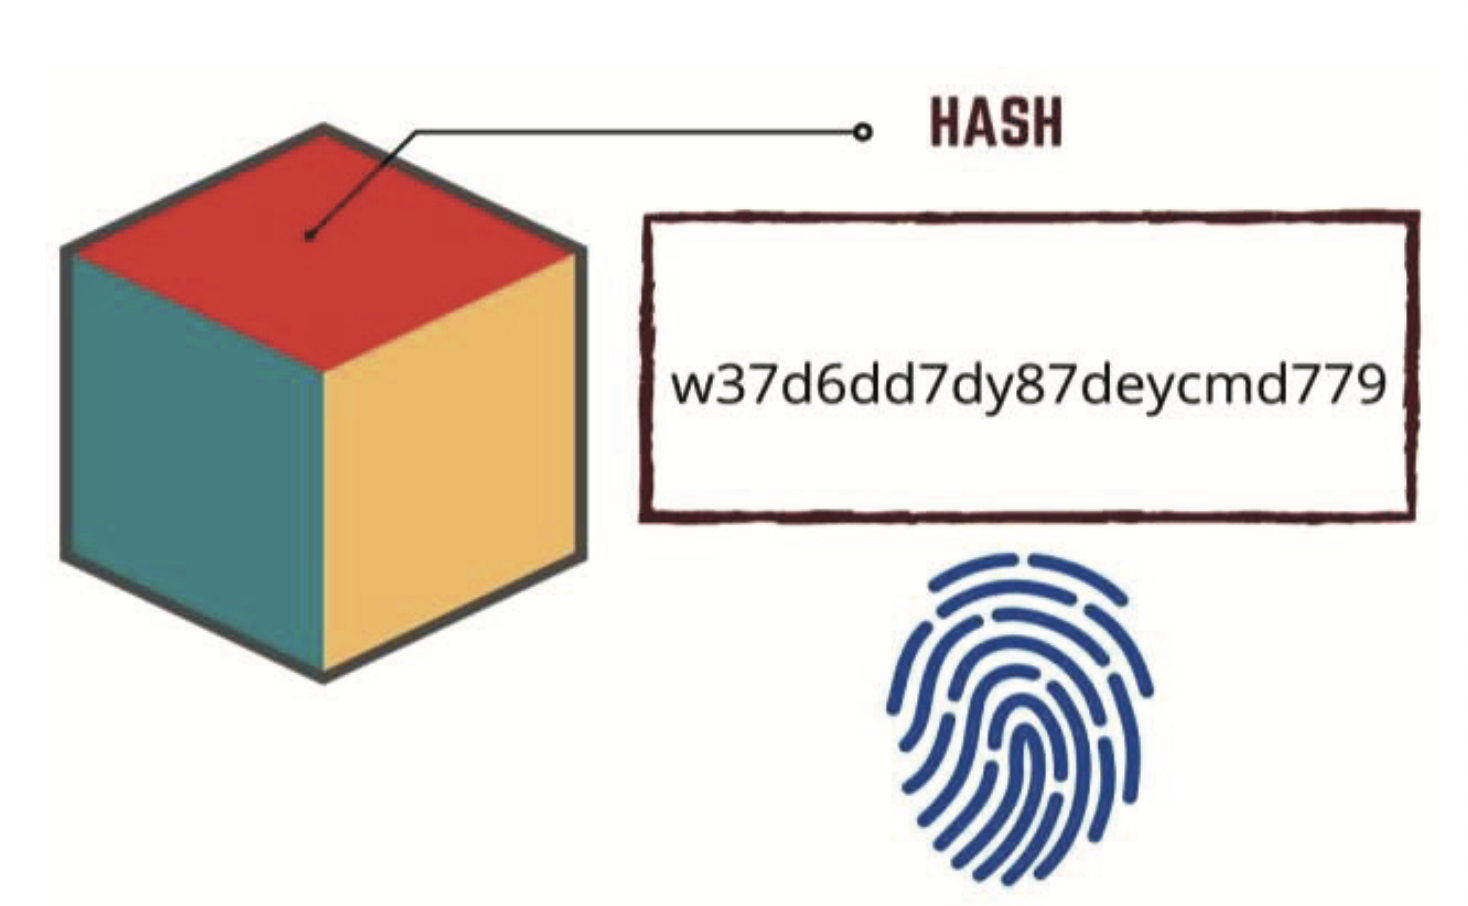
\includegraphics[width=0.37\textwidth]{Blockchain-hash.png} 
  \caption{Blockchain Hash\cite{Jain:Criminal:record}}
\end{wrapfigure} 
Blockchain according to Jarot Sembodo Suroso\cite{Suroso:SKCK} is a decentralized computer software featuring a database that acts as a global ledger, accessible across a network of Bitcoin users who operate on a peer-to-peer basis, adhering to a predefined protocol. Peer- to-peer connects from one computer to another in a large network of all Bitcoin users. To connect to Blockchain a cryptographic identity is required to access it, an email and a password. After a transaction the data cannot be changed because the data is assigned to a block. If someone wants to make adjustments for anything on the Blockchain, they would have to change every block on the Blockchain, this is  the reason why this is impossible. Because all of the network users would have to agree. Blockchain also records a chronological history of all transactions which have occurred in a series of block connected to each other.\cite{Suroso:SKCK}

\subsection{Evolution path of Blockchain}\label{evolution}
\begin{figure}[h]
    \centering
    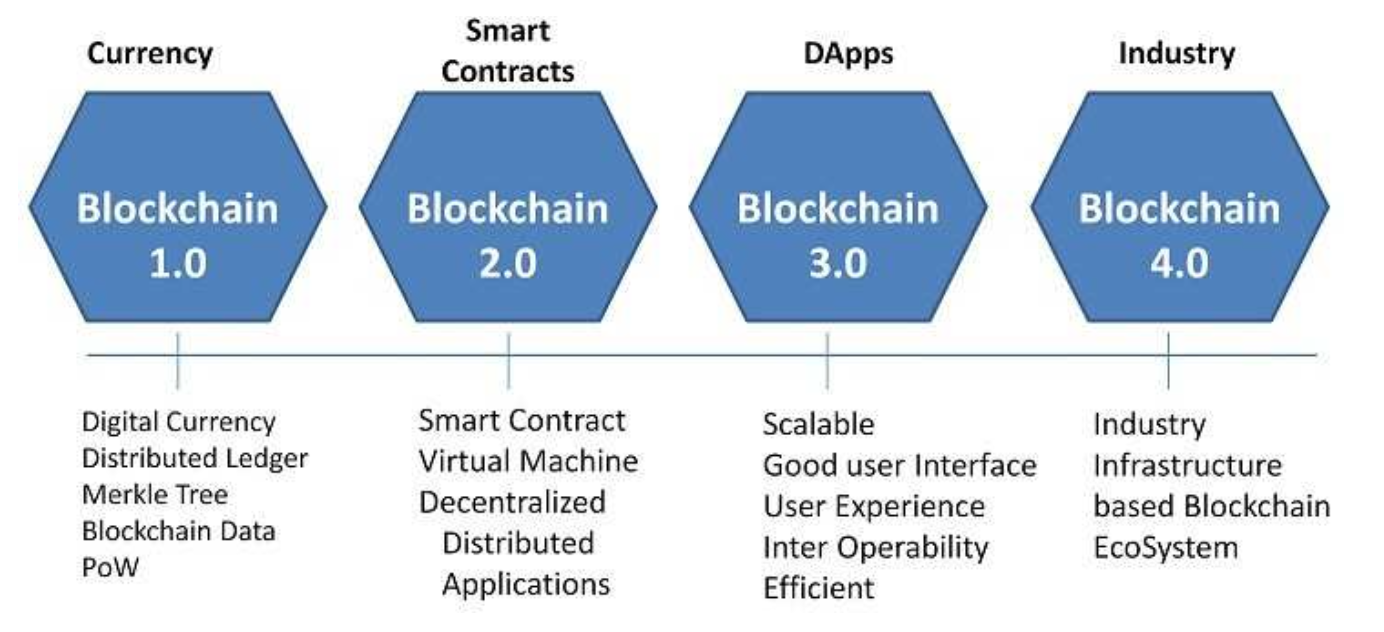
\includegraphics[scale=0.4]{Blockchain-evolution.png}
    \caption{Blockchain Evolution Path \cite{Suroso:SKCK}}
    \label{histogram}
\end{figure}
\paragraph{Blockchain 1.O}
The application of Distributed Ledger Technology (DLT) released cryptocurrency Bitcoin.
\cite{Suroso:SKCK}
\paragraph{Blockchain 2.O}
The Smart Contract feature was introduced as a solution to address the limitations of Blockchain 1.0.
\cite{Suroso:SKCK}
\paragraph{Blockchain 3.0}
At this time Decentralized apps were introduced by the first time. 
\cite{Suroso:SKCK}
\paragraph{Blockchain 4.0}
Leveraging the capabilities of previous version to address the requirements of Industry 4.0 that focuses on trust, privacy, automation, and seamless system integration.
\cite{Suroso:SKCK}

\subsection{Blockchain security standardization} %ešte neviem či tento paragraf bude použitý v záverečnej práci
Like I said in the beginning, our data are never safe, so here comes the question is there a technology that will secure data enough not to be leaked or altered. And the simple answer is yes, Blockchain, thanks to its evolution I mentioned in ~\ref{evolution}.

Even though Blockchain in the last few years have had many unique cyber-attacks, it can withstand most of the attacks. But some of them were successful, this is why there become international standards for Blockchain security:\cite{Xiaofen:Blockchain-security}
\begin{enumerate}
    \item Security threats of distributed ledger technology\cite{Xiaofen:Blockchain-security}
    \item Security framework for distributed ledger technology\cite{Xiaofen:Blockchain-security}
    \item Security guidelines for using distributed ledger technology for decentralized \cite{Xiaofen:Blockchain-security}identity management\cite{Xiaofen:Blockchain-security}
    \item Security assurance for distributed ledger technology\cite{Xiaofen:Blockchain-security}
    \item Security threats and requirements for digital payment services based on distributed ledger technology\cite{Xiaofen:Blockchain-security}
    \item Security threats to online voting systems~\ref{voting} using distributed ledger technology\cite{Xiaofen:Blockchain-security}
    \item Security requirements for digital integrity proofing service based on distributed ledger technology\cite{Xiaofen:Blockchain-security}
    \item Security threats and requirements for data access and sharing based on distributed ledger technology\cite{Xiaofen:Blockchain-security}
\end{enumerate}
   
  
\section{Usecases of Blockchain}\label{Blockchain}
\subsection{Blockchain based criminal record database}
\begin{wrapfigure}{r}{0.5\textwidth}
    \centering
    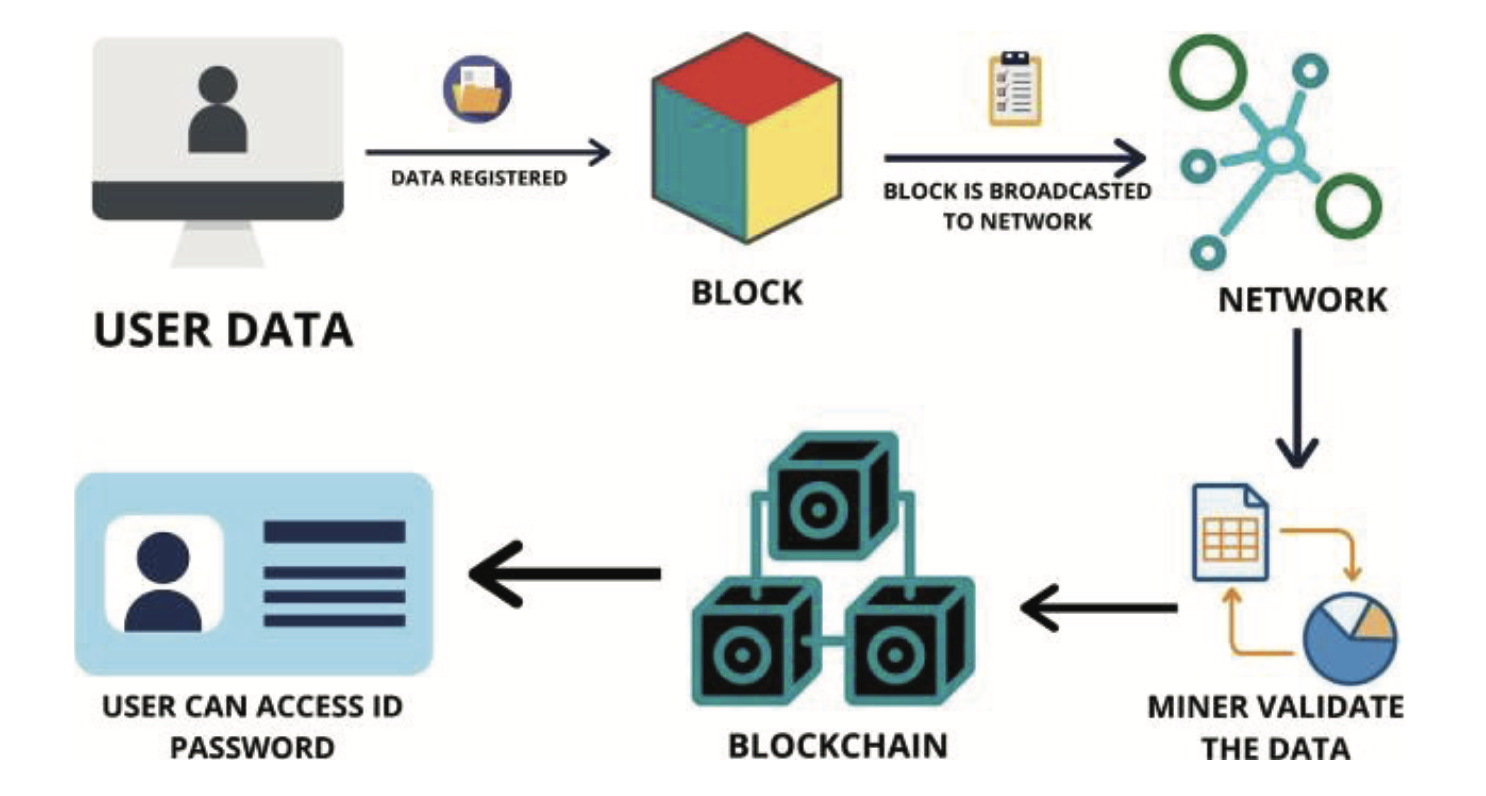
\includegraphics[scale=0.2]{Implemantation of criminal records database.png}
    \caption{Working of the system\cite{Jain:Criminal:record}}
    \label{histogram}
\end{wrapfigure}
The implementation of Blockchain in practice can be for example to manage police records. Basically how it works, everything start with a user reporting a crime, corresponding with an authority officer. This worker then uploads the data on the Blockchain, and a block is created from the gathered information. This block is then uploaded to the Blockchain and everyone on this peer to peer network is alerted about the creation of this block. Right after that there comes an phase of validation, and basically after the validation the data is stored on the Blockchain. It can be accessed just by authorized people with a correct password information. Through logging with the unique password and id the authorized person can add information in a case of a trial or any  other investigation process. This is very convenient and secure type of storing information and surely it is the future of storing criminal records.
\cite{Jain:Criminal:record}
There is a similar system for making Police Record Certificates in SKCK (Surat Keterangan Catatan Kepolisian) in Indonesia. Where they manage the data pretty much the same way but they use a website where they log in and through this website they upload criminal data on the Blockchain, after successful upload the website shows a confirmation. This is the basic understanding of how it works and can work in the Industry 4.0, however not many governments have implemented it yet. But it is very necessary to  do so in the future because it avoids frauds which are not possible thanks to the Blockchain verification.
\cite{Suroso:SKCK}

\subsection{Decentralized E-voting}\label{voting}
In all Democratic countries elections play a huge role. In the elections we are used to, we use so many papers, which are wasted, and some people have to go through the votes count them manually, and release the results to the public. This process takes a lot of time and waste, and there can also be some invalid votes because of a mistake that someone has made during the voting process. And mainly they lack the security and transparency. Every problem I stated can be solved thanks to Blockchain. Blockchain offers the best environment for electronic elections. 
\newline
One of the benefits of E-voting is that people can vote from anywhere with just access to the internet which would be easier for those who live abroad but also from the point of view of a modern person. But with that also comes a lot of security risks. \cite{Sharma:E-voting}



\subsubsection{What should Blockchain based voting system fulfill?}

\paragraph{Anonymity and privacy:}
All the users are unidentified in the transaction of any data in the system \cite{Alvi:E-voting}
\paragraph{Integrity:}
Using Markle tree proof any voting transaction can be checked.
\cite{Alvi:E-voting}
\paragraph{Security:}
It is almost impossible to change a vote because of the Blockchain based hash system
\cite{Alvi:E-voting}
\paragraph{Verifiability:}
Through Smart Contracts the voter with the assigned id can check whether his vote was counted or not
\cite{Alvi:E-voting}
\paragraph{Fairness:}
All the votes are encrypted until the results are released
\cite{Alvi:E-voting}



\subsubsection{Conclusion}
In my opinion, this would make a bunch of things easier, and it would be interesting to have electronic elections. In my opinion, many countries are ready to make a step forward and start testing this kind of technology, but in Slovakia, there is still time for that. There would be many problems with the votes of elderly people because most of them are technologically uneducated.

\subsection{Blockchain in healthcare}
Another institution where Blockchain can be value-able is Healthcare. Concretely the protecting personal patient information. Nowadays patient data are written on the paper 
\cite{Ramar:Healthcare}

\section{Conclusion}
Few sentences to conclude everything



\newpage
\bibliography{literatura}
\bibliographystyle{abbrv}
\end{document}
